%!TEX program = pdflatex
\documentclass{beamer}

%\useoutertheme[glossy]{wuerzburg}
\useinnertheme[shadow,outline]{chamfered}
%\usecolortheme{shark}
\usecolortheme{beaver}
\beamertemplatenavigationsymbolsempty

\usefonttheme{professionalfonts}
\let\digamma\relax
\usepackage[scale=0.85,stdmathitalics=true,romanfamily=casual]{lucimatx}
\usefonttheme[stillsansseriftext]{serif}

\usepackage{bm}


\usepackage{fancyvrb}



\usepackage{textfit} % commands \scaletoheight{height}{text} and \scaletowidth{width}{text}

\usepackage{tikz}

\usepackage{tcolorbox}

\newtheorem{Alert}{Alert}
\newtheorem{Highlight}{Highlight}

\newcommand{\Species}[1]{{\rmfamily \itshape #1}}
\newcommand{\Real}{\ensuremath{\mathbb{R}}}
\newcommand{\RealN}{\ensuremath{\mathbb{R}^n}}
\newcommand{\RealP}{\ensuremath{\mathbb{R}^p}}
\newcommand{\Mtx}[1]{\ensuremath{\bm{#1}}}
\newcommand{\Inv}[1]{\ensuremath{#1^{-1}}}
\newcommand{\InvMtx}[1]{\ensuremath{\bm{#1}^{-1}}}
\newcommand{\Red}[1]{\textcolor{red}{#1}}
\newcommand{\PsInv}[1]{\ensuremath{\bm{#1}^{+}}}

\usepackage{booktabs}



% --- Macro \xvec
% From a tex.stackexchange.com answer by Todd Lehman
% http://tex.stackexchange.com/questions/44017/dot-notation-for-derivative-of-a-vector
\makeatletter
\newlength\xvec@height%
\newlength\xvec@depth%
\newlength\xvec@width%
\newcommand{\xvec}[2][]{%
  \ifmmode%
    \settoheight{\xvec@height}{$#2$}%
    \settodepth{\xvec@depth}{$#2$}%
    \settowidth{\xvec@width}{$#2$}%
  \else%
    \settoheight{\xvec@height}{#2}%
    \settodepth{\xvec@depth}{#2}%
    \settowidth{\xvec@width}{#2}%
  \fi%
  \def\xvec@arg{#1}%
  \def\xvec@dd{:}%
  \def\xvec@d{.}%
  \raisebox{.2ex}{\raisebox{\xvec@height}{\rlap{%
    \kern.05em%  (Because left edge of drawing is at .05em)
    \begin{tikzpicture}[scale=1]
    \pgfsetroundcap
    \draw (.05em,0)--(\xvec@width-.05em,0);
    \draw (\xvec@width-.05em,0)--(\xvec@width-.15em, .075em);
    \draw (\xvec@width-.05em,0)--(\xvec@width-.15em,-.075em);
    \ifx\xvec@arg\xvec@d%
      \fill(\xvec@width*.45,.5ex) circle (.5pt);%
    \else\ifx\xvec@arg\xvec@dd%
      \fill(\xvec@width*.30,.5ex) circle (.5pt);%
      \fill(\xvec@width*.65,.5ex) circle (.5pt);%
    \fi\fi%
    \end{tikzpicture}%
  }}}%
  #2%
}
\makeatother

% --- Override \vec with an invocation of \xvec.
\let\stdvec\vec
\renewcommand{\vec}[1]{\xvec[]{\bm{#1}}}
% --- Define \dvec and \ddvec for dotted and double-dotted vectors.
\newcommand{\dvec}[1]{\xvec[.]{#1}}
\newcommand{\ddvec}[1]{\xvec[:]{#1}}


\usepackage{pifont}
\newcommand{\weblink}{\ding{43}}  % hand with pointing finger

\definecolor{links}{HTML}{2A1B81}
\hypersetup{colorlinks,linkcolor=,urlcolor=magenta}

\usepackage[inline]{asymptote}
\usepackage{attachfile2}
\usepackage{asyfig}



%===========================================================
% Title Info
\title{Scientific Computing for Biologists}
\subtitle{Linear Regression} % (optional)
\date{}
\author[P. Magwene]{Instructor: Paul M. Magwene}


\begin{document}
%===========================================================
\begin{frame}
\titlepage
\end{frame}


%===========================================================
\begin{frame}
  \frametitle{Bivariate Regression: Variable Space Representation}

\begin{figure}
{\centering 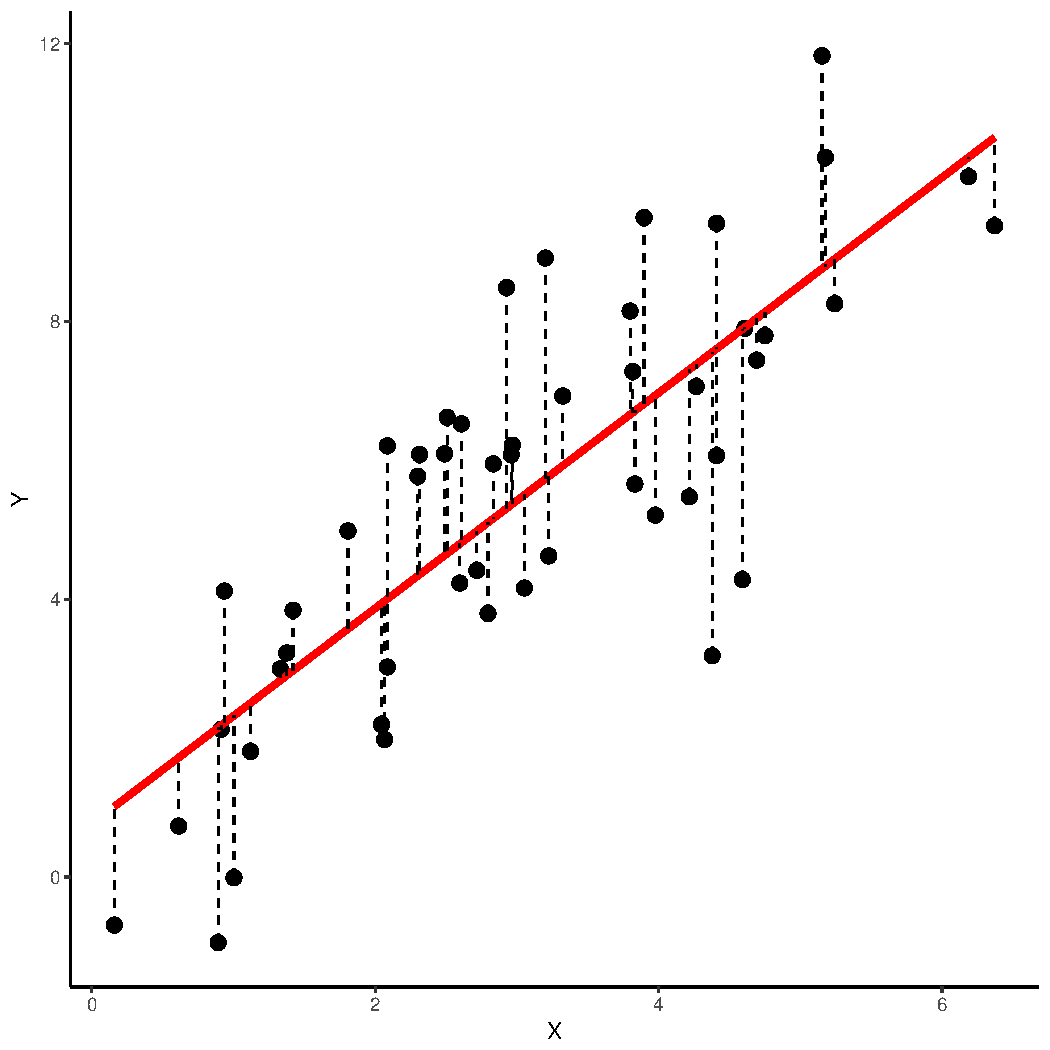
\includegraphics[height=1.75in]{bivariate-regression-image.pdf}}
\end{figure}

\smallskip

The standard bivariate regression equation relating one observed variable $X$ (the predictor) to another observed variable of interest, $Y$ (the outcome) is usually written as:
\[
\widehat{Y} = a + bX.
\]
where $\widehat{Y}$ is the predicted value of $Y$ and $a$ (intercept) and $b$ (slope) are  chosen to minimize $\sum (Y_i - \hat{Y}_i)^2$.


\end{frame}
%===========================================================


%===========================================================
\begin{frame}
  \frametitle{Geometry of Bivariate Regression}

  In vector geometric terms, \emph{regression is projection}! Consider the regression formula for mean-centered vectors:
\[
  \widehat{Y} = bX
\]
  
In vector terms we can view this as:

\begin{center}

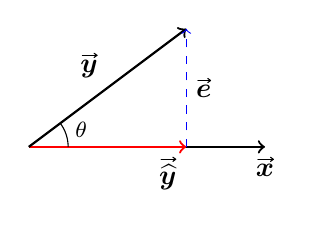
\begin{tikzpicture}[x=0.5cm, y=0.5cm]

\draw[thick,->] (0,0) -- (6,0);
\draw (6,0) node[below] {$\vec{x} $};

\draw[thick,red,->] (0,0) -- (4,0);
\draw (4,0) node[below left] {$\vec{\widehat{y}}$};

\draw[thick,->] (0,0) -- (4,3);
\draw (2,1.5) node[above left] {$\vec{y}$};

\draw[dashed,blue,->] (4,0) -- (4,3);
\draw (4,1.5) node[right] {$\vec{e}$};

\draw (0,0) +(0:0.5cm) arc (0:37:0.5cm);
\path (0,0) ++(18:0.7cm) node[font=\footnotesize] {$\theta$};

\end{tikzpicture}
\end{center}

$\widehat{y}$ is the closest vector to $\vec{y}$ in the subspace defined by $\vec{x}$, i.e. it is the scalar multiple of $\vec{x}$ that minimizes $|\vec{e}|$ 

\[
\widehat{y} = P_{\vec{x}}(\vec{y}) =  \left(\frac{\vec{x} \cdot \vec{y}}{\vec{x} \cdot \vec{x}}\right) \vec{x}
\]







\end{frame}
%===========================================================

\begin{frame}
  \frametitle{Bivariate regression in vector terms}

For mean centered vectors the regression equation is:

  \[
    \vec{\widehat{y}} = b \vec{x}
  \]

From the previous slide we see that we can solve $b$ as: 
\[
b = \frac{\vec{x} \cdot \vec{y}}{\vec{x} \cdot \vec{x}}
\]
\end{frame}

%===========================================================
\begin{frame}[allowframebreaks]
  \frametitle{Bivariate regression: Alternate formulas for slope}

Regression equation for mean-centered vectors: $\vec{\widehat{y}} = b\vec{x}$

There are multiple, equivalent ways to write the solution for $b$:

%
\begin{align*}
b &= \frac{\vec{x} \cdot \vec{y}}{(\vec{x} \cdot \vec{x})} \\
  &= \frac{\vec{x} \cdot \vec{y}}{|\vec{x}|^2}    \\
  &= \frac{|x||y| \cos \theta}{|x|^2} \\
  &= \cos \theta \frac{|y|}{|x|} \\
  &= r_{XY} \frac{|y|}{|x|} \\
\end{align*}


\end{frame}
%===========================================================



%===========================================================
\begin{frame}
  \frametitle{Geometry of Goodness of Fit}

Geometric interpretation of regression goodness-of-fit:

\begin{center}

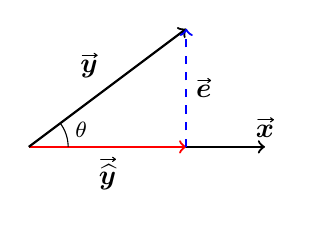
\begin{tikzpicture}[x=0.5cm, y=0.5cm]

\draw[thick,->] (0,0) -- (6,0);
\draw (6,0) node[above] {$\vec{x}$};

\draw[thick,red,->] (0,0) -- (4,0);
\draw (2,0) node[below] {$\vec{\widehat{y}}$};

\draw[thick,->] (0,0) -- (4,3);
\draw (2,1.5) node[above left] {$\vec{y}$};

\draw[thick,dashed,blue,->] (4,0) -- (4,3);
\draw (4,1.5) node[right] {$\vec{e}$};

\draw (0,0) +(0:0.5cm) arc (0:37:0.5cm);
\path (0,0) ++(18:0.7cm) node[font=\footnotesize] {$\theta$};

\end{tikzpicture}

\[
\begin{array}{c}
|\vec{\widehat{y}}|^2 + |\vec{e}|^2 = |\vec{y}|^2
\end{array}
\]

\end{center}

The better the goodness-of-fit, the smaller the angle, $\cos \theta$, and the shorter residual vector, $\vec{e}$.



\end{frame}
%===========================================================

%===========================================================
\begin{frame}
  \frametitle{Geometry of Goodness of Fit}

\begin{figure}
\begin{center}
\subcaptionbox{Good fit}{{\asyinclude[width=0.4\textwidth,keepAspect=true]{good-fit.asy}}}
\subcaptionbox{Bad fit}{{\asyinclude[width=0.4\textwidth,keepAspect=true]{bad-fit.asy}}}
\end{center}
\end{figure}

\end{frame}
%===========================================================


%===========================================================
\begin{frame}
  \frametitle{Bivariate Regression, Goodness of Fit}

How well does our prediction agree with our outcome?

\begin{itemize}
  \item Measure the angle between $\vec{\widehat{y}}$ and $\vec{y}$:
\[
R = \cos \theta_{\vec{y},\vec{\widehat{y}}} = \frac{|\vec{\widehat{y}}|}{|\vec{y}|}
\]

 \item In the single-predictor case $R = r_{XY}$, but this is not generally true when we have multiple predictors.

 \item Note that $|\vec{y}|$ can be expressed as follows:
\begin{eqnarray*}
|\vec{\widehat{y}}|^2 + |\vec{e}|^2 &=& |\vec{y}|^2 \\
SS_\mathrm{regression} + SS_\mathrm{residual} &=& SS_\mathrm{total}
\end{eqnarray*}

 \item With simple substitution we can show that:
\begin{eqnarray*}
SS_\mathrm{regression} &=& R^2 SS_\mathrm{total} \\
SS_\mathrm{residual} &=& (1-R^2)SS_\mathrm{total}
\end{eqnarray*}

\end{itemize}


\end{frame}
%===========================================================



%===========================================================

\begin{frame}
  \frametitle{}

\begin{center}
\begin{Huge}
Regression Models
\end{Huge}
\end{center}
\end{frame}

%===========================================================
\begin{frame}[fragile]
  \frametitle{Variable space view of multiple regression}

\begin{center}
\includegraphics[height=2.5in]{regression-variable-space}
\end{center}


\end{frame}
%===========================================================


%===========================================================
\begin{frame}
  \frametitle{Subject Space Geometry of Multiple Regression}

\begin{center}
\asyinclude[height=2.5in,inline=true]{multiregr.asy}
%\includegraphics[height=2.5in]{multiregr.pdf}

\end{center}
\end{frame}

%===========================================================
\begin{frame}
  \frametitle{Multiple Regression}

Let $Y$ be a vector of values for the outcome variable. Let $\Mtx{X}_i$ be explanatory variables and let $\Mtx{x}_i$ be the mean-centered explanatory variables.
\medskip

$$
\Mtx{Y} = \hat{\Mtx{Y}} + \Mtx{e}
$$
where --
\bigskip

Uncentered version:
$$
\hat{Y} = a\Mtx{1} + b_1\Mtx{X}_1 + b_2\Mtx{X}_2 + \cdots + b_p\Mtx{X}_p
$$

Centered version:
$$
\hat{y} = b_1\Mtx{x}_1 + b_2\Mtx{x}_2 + \cdots + b_p\Mtx{x}_p
$$


\end{frame}
%===========================================================
\begin{frame}
  \frametitle{Statistical Model for Multiple Regression}

In matrix form:

$$
\Mtx{y} = \Mtx{X}\Mtx{b} + \Mtx{e}
$$

$$
\Mtx{y} = \left[ \begin{array}{c}
y_1 \\ y_2 \\ \vdots \\y_n \\
\end{array}
\right]
\;
;
\;
\Mtx{X} = \left[ \begin{array}{ccccc}
1 & x_{11} & x_{12} & \cdots & x_{1p} \\
1 & x_{21} & x_{22} & \cdots & x_{2p} \\
\vdots & \vdots & \vdots & \vdots & \vdots \\
1 & x_{n1} & x_{n2} & \cdots & x_{np} \\
\end{array}
\right]
\;
;
$$

$$
\Mtx{b} = \left[ \begin{array}{c}
a \\ b_1 \\ b_2 \\ \vdots \\ b_p \\
\end{array}
\right]
\;
;
\;
\Mtx{e} = \left[ \begin{array}{c}
e_1 \\ e_2 \\ \vdots \\e_n \\
\end{array}
\right]
$$

\end{frame}
%===========================================================
\begin{frame}
  \frametitle{Estimating the Coefficients for Multiple Regression}


$$
\Mtx{y} = \Mtx{X}\Mtx{b} + \Mtx{e}
$$
\bigskip

Estimate \Mtx{b} as:
$$
\Mtx{b} = (\Mtx{X}^T \Mtx{X})^{-1}\Mtx{X}^T\Mtx{y}
$$

\end{frame}
%===========================================================
\begin{frame}
  \frametitle{Multiple Regression Loadings}


The regression \textbf{loadings} should be examined as well as the regression coefficients.

\begin{center}
\asyinclude[viewportwidth=0.3\textwidth,height=1.5in,keepAspect=true,inline=true]{multiregr-loadings.asy}
%\includegraphics[height=1.5in]{multiregr-loadings.pdf}
\end{center}

Loadings are given by:
		\[
		\cos \theta_{\vec{x_j},\vec{\widehat{y}}} = \frac{\vec{x_j} \cdot \vec{\widehat{y}}}{|\vec{x_j}||\vec{\widehat{y}}|}
		\]


\end{frame}




%===========================================================
\begin{frame}
  \frametitle{Multiple regression: Cautions and Tips}


\begin{itemize}
    \item Comparing the size of regression coefficients only makes sense if all the predictor variables have the same scale
	\item The predictor variables  (columns of $\Mtx{X}$) must be linearly independent; when they're not the variables are \textbf{multicollinear}
	\item Predictor variables that are \textbf{nearly multicollinear} are, perhaps, even more difficult to deal with
\end{itemize}

\end{frame}

%===========================================================

\begin{frame}
  \frametitle{Why is near multicollinearity of the predictors a problem?}

\begin{figure}
\begin{center}
\subcaptionbox{Non-collinear predictors}{\asyinclude[height=1.35in,keepAspect=true]{regr-noncolinear.asy}}
%{\includegraphics[height=1.25in]{regr-noncolinear.pdf}}
\subcaptionbox{Nearly collinear predictors}{\asyinclude[height=1.35in,keepAspect=true]{regr-colinear.asy}}
%{\includegraphics[height=1.25in]{regr-colinear.pdf}}
\end{center}
\caption{When predictors are nearly collinear, small differences in the vectors can result in large differences in the estimated regression.}
\end{figure}


\end{frame}

%===========================================================

\begin{frame}
  \frametitle{What can I do if my predictors are (nearly) collinear?}

\begin{itemize}
	\item Drop some of the linearly dependent sets of predictors.
	\item Replace the linearly dependent predictors with a combined variable.
	\item Define orthogonal predictors, via linear combinations of the original variables (PC regression approach)
	\item `Tweak' the predictor variables so that they're no longer multicollinear (Ridge regression).
\end{itemize}


\end{frame}




%===========================================================
\begin{frame}
  \frametitle{Curvilinear Regression}

Curvilinear regression using \textbf{polynomial models} is simply multiple regression with the $x_i$ replace by powers of $x$.
\bigskip

$$
\hat{y} = b_1\Mtx{x} + b_2\Mtx{x}^2 + \cdots + b_p\Mtx{x}^n
$$

\medskip

Note:
\begin{itemize}
	\item this is still a \emph{linear} regression (linear in the coefficients)
	\item best applied when a specific hypothesis justifies there use
	\item generally not higher than quadratic or cubic
\end{itemize}

\end{frame}
%===========================================================
\begin{frame}[fragile]
  \frametitle{Example of Curvilinear Regression}

\begin{center}
\includegraphics[height=1.75in]{curvilinear}\\
 $\Mtx{y} = 3\Mtx{x} + 0.5\Mtx{x}^2 + \Mtx{e}$
\end{center}

\begin{Rcode}
lm(formula = y ~ x + I(x^2))
Coefficients:
            Estimate Std. Error t value Pr(>|t|)
(Intercept)  0.02229    0.11651   0.191    0.849
x            2.94001    0.09693  30.331  < 2e-16 ***
I(x^2)       0.47146    0.07685   6.135 1.68e-07 ***
\end{Rcode}


\end{frame}


%===========================================================

\begin{frame}
  \frametitle{Least Squares Regression vs. Major Axis Regression}
\begin{center}
\includegraphics[width=4in]{ols_vs_majoraxis}
\end{center}
\end{frame}


%===========================================================


\begin{frame}
  \frametitle{Vector Geometry of Major Axis Regression}

\begin{figure}
\begin{center}
\subcaptionbox{OLS}{{\asyinclude[height=1.05in,keepAspect=true]{geom-OLS.asy}}}
%{\includegraphics[height=1.05in]{geom-OLS.pdf}}
\subcaptionbox{Major Axis Regression}{{\asyinclude[height=1.05in,keepAspect=true]{geom-majaxis.asy}}}
%{\includegraphics[height=1.05in]{geom-majaxis.pdf}}
\end{center}
\caption{Vector geometry of ordinary least-squares and major axis regression.}
\end{figure}


\end{frame}

%===========================================================





\end{document}


%===========================================================
\begin{frame}
  \frametitle{Two-group ANOVA as Regression}

We can also use a geometric perspective to test whether the mean of a variable differs between two groups of subjects.

\begin{itemize}
\item Setup a `dummy variable' as the predictor $X_g$.   We assign all subjects in group 1 the value 1 and all subjects in group 2 the value -1 on the dummy variable.  We then regress the variable of interest, $Y$, on $X_g$.

\end{itemize}
%
$$
\Mtx{y} = \Mtx{X}_g\Mtx{b} + \Mtx{e}
$$
%
\begin{figure}
{\centering 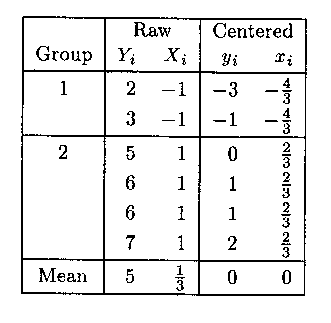
\includegraphics[height=1.5in]{anova-2group-table.pdf}}
\end{figure}


\end{frame}
%===========================================================


%===========================================================
\begin{frame}
  \frametitle{Two-group ANOVA as Regression, cont}

\begin{itemize}

\item When the means are different in the two groups, $X_g$ will be a good predictor of the variable of interest, hence $\vec{y}$ and $\vec{x_g}$ will have a small angle between them.

\item When the means in the two groups are similar, the dummy variable will not be a good predictor.  Hence the angle between $\vec{y}$ and $\vec{x_g}$ will be large.

\end{itemize}

\begin{center}

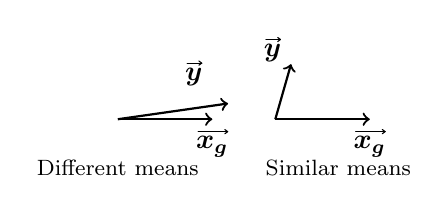
\begin{tikzpicture}[x=0.2cm, y=0.2cm]

% different means
\draw[thick,->] (-10,0) -- (-4,0);
\draw (-4,0) node[below] {$\vec{x_g}$};

\draw[thick,->] (-10,0) -- (-3,1);
\draw (-4,1.5) node[above left] {$\vec{y}$};
\draw (-10,-2) node[below,font=\footnotesize] {Different means};

% Similar means
\draw[thick,->] (0,0) -- (6,0);
\draw (6,0) node[below] {$\vec{x_g}$};

\draw[thick,->] (0,0) -- (1,3.5);
\draw (1,3) node[above left] {$\vec{y}$};
\draw (4,-2) node[below,font=\footnotesize] {Similar means};

\end{tikzpicture}

\end{center}

\end{frame}
%===========================================================




